%%%%%%%%%%%%%%%%%%%%%%%%%%%%%%%%%%%%%%%
%----------------------------------------     算法     ---------------------------------------%
%%%%%%%%%%%%%%%%%%%%%%%%%%%%%%%%%%%%%%%
\chapter{算法}
本文希望通过分析移动应用开发者的需求,为其推荐高质量、功能相关的第三方库,以协助其快速开发优质的移动应用,从而吸引用户并增加收益。本文从移动应用开发流程的两个阶段入手,即需求分析和后期维护,分析获取开发者的需求。具体而言,在需求分析阶段,主要利用移动应用的描述作为输入信息,通过分析描述这一文本数据,从而提出其中所包含的移动应用的功能信息;在后期维护阶段,由于已经有早期开发的移动应用的版本,因此该版本所包含的功能信息可以从其视图界面、程序代码等方面获取。所提取的功能信息均用以表征开发者的需求,从而可以通过聚类的方法,将相似功能的移动应用聚集到一起。所聚集的移动应用具有很强的相似性,相似的移动应用可以为开发者提供参考和借鉴,特别是质量较好、评分较高的移动应用,其所使用的第三方库便是可以为开发者提供参考之处。通过该方法分析获得的第三方库,是开发者所需的且优质的第三方库,因而可以推荐给开发者使用。

本章将对本文研究的问题作具体定义,明确问题的背景及目标,详细内容将在4.1节中阐述。在明确研究问题的目标后,本章将针对研究问题给出本文的解决方法。解决方法包括三分部分:相似性计算、移动应用聚类、第三方库推荐,算法的整体框架将在4.2节中详细阐述。其中,相似性计算将根据移动应用开发流程的不同阶段,对不同的信息源进行分析计算。在需求分析阶段,本文将通过分析移动应用的描述来获取功能需求,因而需对描述文字进行自然语言处理和分析,并依此计算移动应用(功能)的相似性,具体计算方法将在4.3节中阐述。在后期维护阶段,本文将通过分析现有版本的移动应用的视图界面来获取功能信息,因而需对移动应用的程序包文件进行处理,并从程序代码层面对移动应用内部信息进行分析,从而计算移动应用间的相似性,具体实现算法将在4.4节中详细描述。基于计算获得的移动应用的相似性,本文使用聚类算法把功能相似的移动应用聚集到一起,聚类算法和过程将在4.5节中阐述。最后,本文的最终目标——为开发者推荐优质可靠的第三方库——将在4.6节中展开讨论,基于前两部分的相似性计算和移动应用聚类,本文可以准确地定位开发者的需求,并根据相似移动应用使用第三方库的情况,为开发者匹配最佳的第三方库。下文将对以上几个部分内容分别展开讨论。



%%%%%%%%%%%%%%%%%%%%%%%%%%%%%%%%%%%%%%%
%----------------------------------------     问题定义     ---------------------------------------%
%%%%%%%%%%%%%%%%%%%%%%%%%%%%%%%%%%%%%%%
\section{问题定义}
本文主要研究的问题是为移动应用开发者推荐优质、合适的第三方库。因此,需要对移动应用和第三方库,以及相关问题进行定义。首先,给定移动应用集合$\mathcal{A}$,其中任意一个移动应用为$\mathbf{a}_i \in \mathcal{A}$。为了协助开发者寻找最合适的第三方库,则需要对开发者的需求进行分析。本文分别对两个不同阶段的需求进行分析,分析内容包括移动应用描述和视图信息。对于任意一个移动应用$\mathbf{a}_i$,其描述的文本信息表示为$\mathbf{t}_i$,视图信息表示为$\mathbf{v}_i$,则移动应用可表示为由描述和视图组成的特征集合$\mathbf{a}_i = \{\mathbf{t}_i, \mathbf{v}_i\}$。由于描述和视图属于两个不同的开发阶段,因此本文在对移动应用实际操作过程中,分别表示为$\mathbf{a}_i = \{\mathbf{t}_i\}$和$\mathbf{a}_i = \{\mathbf{v}_i\}$。但此两项特征的基本概念和依据相同,故在此不做区分。

对开发者需求的分析,本文是通过搜寻相似移动应用的方式来解决的。具体而言,为给开发者推荐第三方库,本文先对移动应用市场上已有的移动应用进行分析,了解统计不同类别、不同功能的移动应用所使用的第三方库情况。一个移动应用可能使用多个第三方库。例如,一个常用的社交移动应用,其可能使用的第三方库包括聊天界面展示、定位服务、数据库管理等。因此,对任意一个第三方库定义为$l_j \in \mathcal{L}$,其中$\mathcal{L}$为所有移动应用可能使用的第三方库集合。那么,一个移动应用所使用的第三方库可以表示为$\mathbf{l}_i = \{l_{i,1}, l_{i,2}, ..., l_{i,n}\}$。在此基础上,本文将与开发者需求相近的移动应用筛选出来,这些移动应用所使用的第三方库便进入后续推荐的候选名单。因此,在搜寻相似移动应用的过程中,本文定义移动应用相似性如下:
\begin{definition}[移动应用相似性]
给定一个移动应用集合$\mathcal{A}$,移动应用相似性计算的目标函数为$f:\mathcal{A} \times \mathcal{A} \rightarrow \mathbb{R_+}$,其中$f(\mathbf{a}_i, \mathbf{a}_j)$表示移动应用$\mathbf{a}_i$与$\mathbf{a}_j$间的相似性。
\end{definition}

为了筛选相似的移动应用,通常的解决方法是将功能相近的移动应用进行聚类。因此,本文根据移动应用的相似性,对其进行聚类操作,聚类过程将在4.5节详细阐述。聚类后的移动应用将被分成$k$个集合,表示为$\mathcal{S} = \{S_1, S_2, ..., S_k\}$,每个集合中的移动应用互相间都具有相似的功能。因此,相应集合中的移动应用所使用的第三方库同样呈现类似的关系。最终,研究问题转化成如何从一组功能相似的移动应用中找到对开发者有用的第三方库。就该问题,本文根据开发者所需开发的移动应用$\mathbf{a}_t$所在集合$S_i$(聚类后的所在集合),使用协同过滤算法,筛选出最可能被开发者采纳的第三方库,并将此列表推荐给开发者。至此,本文整个研究问题已定义清楚,下面将详细介绍本文对各个问题的具体解决方案和步骤。



%%%%%%%%%%%%%%%%%%%%%%%%%%%%%%%%%%%%%%%
%----------------------------------------     算法框架     ---------------------------------------%
%%%%%%%%%%%%%%%%%%%%%%%%%%%%%%%%%%%%%%%
\section{算法框架}
\begin{figure}
	\centering
	\includegraphics[width=5.7in]{figures/architecture}
	\caption{TV-LibRec算法整体框架结构图。}
\end{figure}

针对本文的研究问题——为移动应用开发者推荐最合适的第三方库,本文提出了一种基于文本和视图相似性的第三方库推荐算法(TV-LibRec: \textbf{Lib}rary \textbf{Rec}ommendation based on \textbf{T}extual and \textbf{V}iew similarities),算法的整体框架如图4-1所示。

从框架图中可以看到,针对开发者即将开发的或需要优化的移动应用,算法分别从其文本(描述)和视图(界面代码)两个层面提取移动应用功能信息。由于文本和视图分别代表两个不同的开发阶段,因此在算法实际应用过程中将独立执行,分别为T-LibRec和V-LibRec。而在聚类和推荐部分,两阶段的算法基本一致,因此不作区分。图4-1左侧是对文本信息的处理,本文从Google Play上爬取了移动应用的描述信息,通过对描述的文本清理和特征提取,可以从中抽取与移动应用功能相关的特征信息,具体算法将在4.3节中阐述。图4-1右侧是对移动应用视图信息的获取,本文通过分析移动应用的用户界面布局、图片、列表等视图信息,并从程序代码中抽取对应特征,从而构建移动应用在视图上的特征,详细描述将在4.4节中展开。

本文建立了一个移动应用数据库,其中包含了大量从Google Play上爬取的移动应用描述和程序包。数据库中的移动应用都已使用本文提出的聚类算法,根据移动应用间的文本和视图相似性进行提前聚类。因此,对于一个开发者所需的移动应用而言,可以通过相似性计算方法,找到与其相关的簇,这将大大降低与数据库中每个移动应用计算相似性的频率,从而提高整体算法效率。本文提出的对移动应用聚类的算法在4.5节中阐述。

在找到开发者所需移动应用所在的簇之后,从图4-1最后一个流程框图中可以看到,本文将为开发者推荐合适的第三方库。该过程分为三个步骤:首先,从所在簇中筛选出与目标移动应用最为相似的一组移动应用;其次,在这些移动应用中查找其所使用的第三方库;最后,根据这些移动应用所使用的第三方库情况为开发者推荐。具体的推荐算法和过程将在4.6节中详细阐述。

如上文所述,本文提出的TV-LibRec第三方库推荐算法一共分为三个部分。特别的,在第一部分中,又根据实际开发流程分为两个不同的子方法。根据图4-1可以清晰地了解TV-LibRec算法的整体流程,下文将分别对每个部分的实现方法和过程进行深入阐述。



%%%%%%%%%%%%%%%%%%%%%%%%%%%%%%%%%%%%%%%
%--------------------------------------     文本相似性     ------------------------------------ -%
%%%%%%%%%%%%%%%%%%%%%%%%%%%%%%%%%%%%%%%
\section{文本相似性}
根据移动应用描述的相似性来表征移动应用本身的相似性,是基于描述中包含了移动应用的功能信息,且描述相似体现了功能的相似这一事实。本节将详细阐述对移动应用描述进行文本数据清洗(4.3.1节),将描述文本转化成特征向量(4.3.2节),以及计算移动应用描述相互间的相似性(4.3.3节)。特别的,由于本文的数据均来自Google Play的英文网站,因此研究问题和方法都以英文为对象。


\subsection{数据清洗}
在从描述文本中提取出特征信息前,需要先对描述文本进行基本的自然语言处理操作,即对文本数据进行清洗。具体清洗操作分为两个步骤:过滤和词干提取。下面将详细描述此过程,本文以Facebook移动应用的描述(如图4-2所示)为例子进行阐述。

\begin{figure}
	\centering
	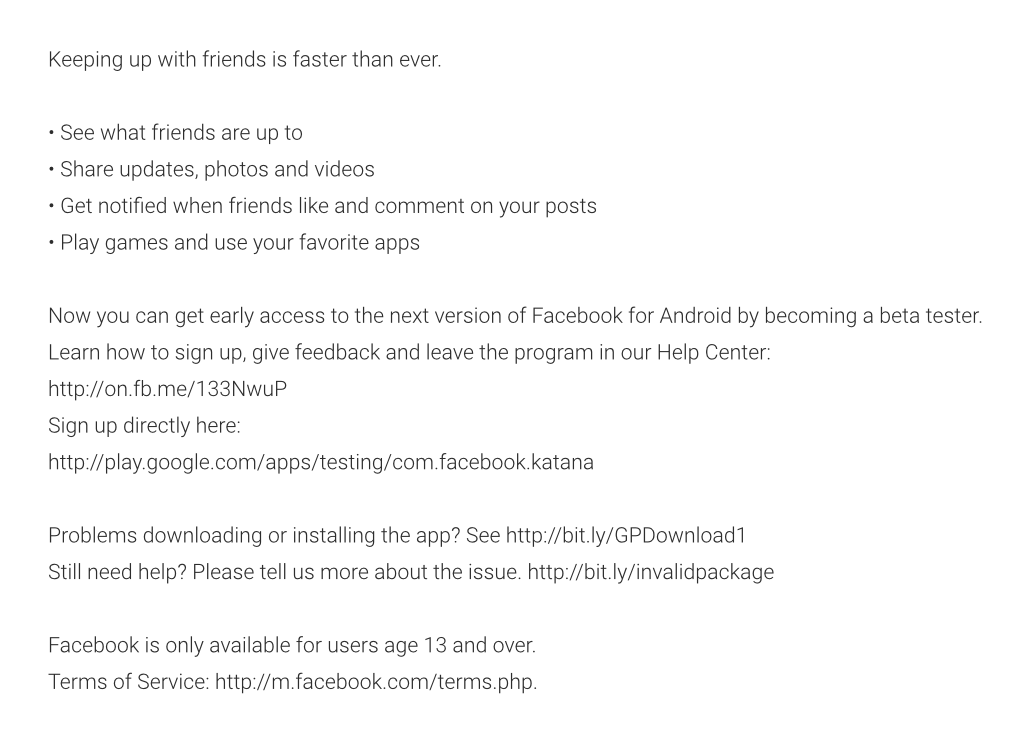
\includegraphics[width=4.7in]{figures/fb_desc}
	\caption{Facebook移动应用描述信息。}
\end{figure}

由于Google Play移动应用商城通常包含多种语言,即使本文以英文为主要研究对象语言,但其中依旧会夹杂其他语言的文字。例如,有些开发者会在发布的移动应用的英文描述最后,加上一两句用开发者本国语言写的相关介绍。该做法通常是为了吸引更多本土用户,也包含其他原因。由于本文研究的问题和方法以英文为对象,因此需要将这些非英语的文字去除。本文利用自然语言处理工具Natural Language Toolkit (NLTK)\cite{nltk}将描述中的非英语部分过滤掉。此外,从图4-2可以观察到,描述文本中通常还会有标点符号、网络链接地址(例如,\texttt{http://on.fb.me/133NwuP})等,同样需要将这些无关信息过滤掉,避免影响后续特征提取。过滤后的描述文本一般只剩下英文单词,图4-3显示了对Facebook移动应用描述过滤后的结果。

\begin{figure}
	\centering
	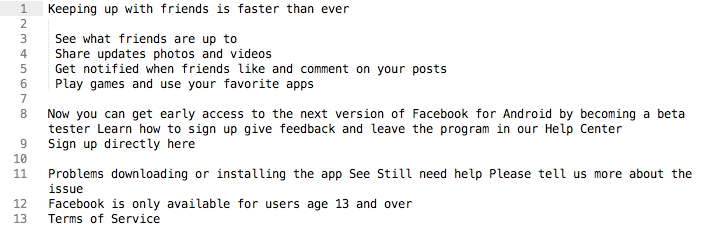
\includegraphics[width=4.7in]{figures/desc_filter}
	\caption{过滤后的Facebook移动应用描述文本。}
\end{figure}

在对描述文本进行过滤操作后,为了抓取文本中最关键的单词,从而理解文本语义信息,本文将描述文本中无关紧要的停用词去除并提取词干。停用词是语言中最常出现的助词、介词、连词等一些单词,其本身不具有特别意义,例如英文中的“the”、“at”、“which”等。本文利用一个停用词列表,将这些并不含有实际意义的单词去除。在去除停用词后,本文需要对描述本文进行词干提取。词干提取是自然语言处理中通用的方法,用以识别单词的词根形式,减少文本中的单词数量。例如,单词“stems”、“stemmer”、“stemming”、“stemmed”都是基于单词“stem”变化形式生成的,因此“stem”是这些单词的词根。由于这些单词虽然在形式上不同,但是其实际语义并无差异,因而在自然语言处理中将这些单词都转化成同一词根表现形式,以减少文本中不同单词的数量,从而提高特征提取效率。在对Facebook移动应用的描述文本进行停用词去除和词干提取后,其最终结果如图4-4所示。

\begin{figure}
	\centering
	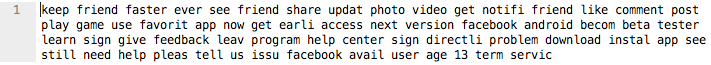
\includegraphics[width=4.7in]{figures/desc_stem}
	\caption{去除停用词并提取词干后的Facebook移动应用描述文本。}
\end{figure}

至此,通过对移动应用描述文本数据的清洗,本文得到了内容更为精简的文本,文本包含了移动应用的功能信息,为下一节特征的抽取做好基础准备。


\subsection{特征抽取}
在上一节描述文本的基础上,本节对描述文本中的文字进行抽象化,提取能够表征文本信息的特征向量。本文使用由Le等提出的Distributed Memory Model of Paragraph Vectors (PV-DM)模型\cite{le2014distributed}(通称doc2vec模型,本文也将采用此名称),将描述的文本内容转化成向量的形式。Doc2vec模型是基于word2vec模型\cite{mikolov2013efficient},通过加入段落向量进行扩充实现的。因此,本文将首先阐述word2vec模型的原理和过程,再在此基础上解释doc2vec模型的原理,最后阐述从移动应用描述中抽取特征的过程。

在自然语言处理研究中,经常需要对单词进行数学表示,称为词向量。通常的表示方法为,单词存在则为1,不存在就为0,这种表示方法被称为one-hot representation。然而,这种表示方法有个极大的缺陷,即词向量中数据极为稀疏。例如,一篇文章有1000个单词,那么每个词向量中只有一个维度的值为1,而其他999个维度都为0值,这对于自然语言处理而言带来了极大的困难。为了解决高维且稀疏的表示问题,研究者将向量低维化实数化,即用维度较少的实数而非高维的布尔值来表示词向量,该表示方法被称为distributed representation。因此,便有了接下来的研究问题——如何将文章中的单词表示成一个低维的实数向量?因为不同于one-hot representation表示方式,distributed representation的词向量无法直接从文章中获得。Mikolov等\cite{mikolov2013efficient}为了解决该问题,借鉴深度学习的思想和方法,提出了word2vec模型。该模型可以高效地学习生成distributed representation的词向量。Word2vec模型分为两种不同实现方式的模型:Continuous Bag-of-Words Model (CBOW)和Continuous Skip-gram Model (Skip-gram)。此两种模型的理论基础相似,只是对调了输入和输出部分。PV-DM模型是由CBOW模型演化而来,因此本文着重阐述CBOW模型(为便于阐述,下文中统一用word2vec来表示)。

Word2vec模型的目标是根据文本中的上下文来预测一个单词。如图4-5所示,word2vec模型是一个三层的神经网络结构,包括输入层、映射层和输出层。输入层由上下文的单词组成。训练伊始,word2vec会使用一个大小适当的移动窗口来抽取单词,该窗口中的单词则处于同一个语境中。若需要对单词$\mathsf{Word_t}$进行学习,那么在该单词前面的其他单词(如$\mathsf{Word_{t-2}}$、$\mathsf{Word_{t-1}}$)则为上文,后面的其他单词(如$\mathsf{Word_{t+1}}$、$\mathsf{Word_{t+2}}$)则为下文,这样便构成了局部的上下文语境。每一个单词都会被映射到一个唯一的词向量,表示为单词矩阵$\mathbf{W}$中的一列,而矩阵中列的下标对应于单词在语料库中的位置。后一层网络,不同于前馈神经网络语言模型(NNLM: Feedforward Neural Net Language Model)\cite{bengio2003neural},word2vec删去了NNLM中非线性的隐藏层,与之替换的是一个由所有单词共享的映射层。因为在神经网络的训练过程中,非线性的隐藏层通常是最复杂最耗时的结构部分,所以word2vec通过简化该部分结构,
\begin{figure}
	\centering
	\includegraphics[width=5.5in]{figures/word2vec}
	\caption{Word2vec模型结构图。}
\end{figure}
从而提高计算效率。Word2vec中的映射层其实是一个上下文词向量整合的过程,通常的操作可以是向量级联(concatenation)或者向量求和(sum)。设单词$\mathsf{Word_t}$用词向量$\mathbf{w}_t$表示,则图4-5中的映射层向量可以表示为:
\begin{equation}
concatenation: \mathbf{w}_p = \mathbf{w}_{t-2} \cup \mathbf{w}_{t-1} \cup \mathbf{w}_{t+1} \cup \mathbf{w}_{t+2}
\end{equation}
\begin{equation}
sum: \mathbf{w}_p = \sum_{\substack{i=t-2 \\ i \neq t}}^{t+2} \mathbf{w}_i
\end{equation}
其中,$\mathbf{w}_p$表示映射后的向量。最后一层是将前一层的映射向量作为特征,构建一个对数线性分类器,即根据输入的特征来对语料库中的单词进行分类,而训练过程即是学习正确分类目标单词的过程。具体的,给定需要训练的单词序列$\{\mathbf{w}_1, \mathbf{w}_2, \mathbf{w}_3, ..., \mathbf{w}_T\}$,word2vec的目标函数即为最大化以下平均对数概率:
\begin{equation}
\frac{1}{T} \sum_{t=k}^{T-k} \log p(\mathbf{w}_t \mid \mathbf{w}_{t-k}, ..., \mathbf{w}_{t+k})
\end{equation}
其中,$T$表示需要训练的单词数量,$p(\cdot)$为单词$\mathbf{w}_t$出现的条件概率值。因此,经过以上对语料库的训练,在预测过程中,只需计算目标单词在所处上下文中的条件概率值,即可得到对应的结果。通常预测的方法是使用例如softmax\cite{christopher2006pattern}这样的多分类器来实现,具体如下:
\begin{equation}
p(\mathbf{w}_t \mid \mathbf{w}_{t-k}, ..., \mathbf{w}_{t+k}) = \frac{e^{y_{\mathbf{w}_t}}}{\sum_i e^{y_i}}
\end{equation}
其中,$y_i$表示输出单词$i$未归一化的对数概率值,其计算方法如下:
\begin{equation}
y = \mathbf{U}h(\mathbf{w}_{t-k}, ..., \mathbf{w}_{t+k}; \mathbf{W}) + \mathbf{b}
\end{equation}
其中,$\mathbf{U}$和$\mathbf{b}$为softmax的参数,$h(\cdot)$是由$\mathbf{W}$中的词向量级联或求和构建而成的。为了对大量单词进行快速训练,因此在实际操作中,word2vec使用hierarchical softmax\cite{morin2005hierarchical}作为输出层的多分类器。因而,输出层实际上是一棵由Huffman树\cite{huffman1952method}构建而成的二叉树,其中每个叶子节点表示语料库中的单词,而单词在语料库中出现的次数则为其所在节点的权重,且每个节点都有唯一的编码。Word2vec对单词的训练过程使用了常见的随机梯度下降方法,梯度值是通过反向传播的方法\cite{rumerhart1986learning}进行计算的。该方法在神经网络训练中大量使用,具体算法可以参见相关文献,在此不做赘述。

\begin{figure}
	\centering
	\includegraphics[width=5.5in]{figures/doc2vec}
	\caption{Doc2vec模型结构图。}
\end{figure}

通过对word2vec模型的分析,可以发现初始随机赋值的输入词向量,在对目标单词预测的过程中,间接地转化成了富含语义的词向量。依据word2vec此特性,doc2vec于是在word2vec的基础上进行扩展,将文档作为向量加入到训练和预测的过程中。如图4-6所示,不仅来自单词矩阵$\mathbf{W}$的每一个词向量作为特征输入,而且每一个文档也被映射到一个向量(表示为文档矩阵$\mathbf{D}$中的一列)作为输入。文档向量与词向量一同作为输入,在影射层中进行级联或求和,来预测语境中的目标单词。此外,对于word2vec中公式(4-5)的$h(\cdot)$函数,将由$\mathbf{W}$中的词向量和$\mathbf{D}$中的文档向量一起构建。特别的,文档向量只在当前文档的语境中共享,即对某一文档进行训练和预测时,仅当前文档向量作为确定输入进行计算,而其他文档向量不参与计算。词向量则不同,整个词向量矩阵$\mathbf{W}$在所有文档的训练和预测中都共享使用。

本文从Google Play市场上爬取了23,398个移动应用的描述,每个描述作为表征移动应用功能的文本,经过4.3.2节的数据清洗,形成23,398个文档。这些文档作为本文实验的语料库,在此基础上进行文档向量的学习。特别的,由于移动应用的描述与日常用词不完全相同,因此本文不使用通用的词汇表对描述文档进行训练,而是利用这两万多个描述文档中出现的词汇作为实际词汇表,在训练和预测过程中作为参照。本文对每个描述文档进行长度为$l$的滑窗扫描,每个窗口中的所有单词将作为上下文语境输入模型。设描述文档矩阵为$\mathbf{T}$,其每列表示描述文档向量$\mathbf{t}_i$,则如上文所述,本文将该向量与描述文档中的每个词向量一起作为doc2vec的输入进行训练和预测。模型收敛后,本文得到一组移动应用描述文档的向量$\mathcal{T} = \{\mathbf{t}_1, \mathbf{t}_2, ..., \mathbf{t}_n\}$。获得了描述文档的向量表征后,本文将在下节中对描述向量进行相似性计算。


\subsection{相似性计算}
在推荐系统中,经常通过分析用户喜好的物品,查找与其具有相似喜好的其他用户,根据其他用户的喜好情况,为目标用户推荐可能喜好的物品。在此推荐过程中,查找相似用户是最为关键的一个步骤,因此计算不同用户间的相似情况成为推荐系统中主要部分之一。常用的相似性计算方法包括欧几里得距离、皮尔森相关系数(PCC: Pearson Correlation Coefficient)\cite{pearson1895note}、余弦相似度(Cosine Similarity)等。本文分别使用皮尔森相关系数和余弦相似度对描述文档的向量计算相似性。

\textbf{皮尔森相关系数:}皮尔森相关系数是对两个变量的线性关系的衡量。用皮尔森相关系数来表示两个移动应用的描述间的相似性,可用以下公式表示:
\begin{equation}
f_{\mathit{PCC}}(\mathbf{t}_i, \mathbf{t}_j) 
= \frac{\sum_{x=1}^\chi (t_{i,x} - \overline{t_i})(t_{j,x} - \overline{t_j})}{\sqrt{\sum_{x=1}^\chi (t_{i,x} - \overline{t_i})^2}\sqrt{\sum_{x=1}^\chi (t_{j,x} - \overline{t_j})^2}}
\end{equation}
其中,$\mathbf{t}_i$和$\mathbf{t}_j$为移动应用的描述向量,$t_{i,x}$表示描述向量$\mathbf{t}_i$中第$x$维数据,$\overline{t_i}$为描述向量$\mathbf{t}_i$各维度的均值,$\chi$是描述向量的长度。$f_{\mathit{PCC}}(\mathbf{t}_i, \mathbf{t}_j)$的取值范围在$[-1,1]$内,若$f_{\mathit{PCC}}>0$,则表示描述向量$\mathbf{t}_i$与$\mathbf{t}_j$具有正相关性;若$f_{\mathit{PCC}}=0$,则表示描述向量间没有相关性;若$f_{\mathit{PCC}}<0$,则说明是负相关。

\textbf{余弦相似度:}余弦相似度是用来衡量两个非零向量间的夹角的余弦值。用余弦相似度来表示两个移动应用的描述间的相似性,可用以下公式表示:
\begin{equation}
f_{\mathit{cos}}(\mathbf{t}_i, \mathbf{t}_j) 
= \frac{\mathbf{t}_i \cdot \mathbf{t}_j}{\parallel \mathbf{t}_i \parallel \parallel \mathbf{t}_j \parallel}
= \frac{\sum_{x=1}^\chi t_{i,x}t_{j,x}}{\sqrt{\sum_{x=1}^\chi t_{i,x}^2}\sqrt{\sum_{x=1}^\chi t_{j,x}^2}}
\end{equation}
其中,$\mathbf{t}_i$和$\mathbf{t}_j$为移动应用的描述向量,$t_{i,x}$表示描述向量$\mathbf{t}_i$中第$x$维数据,$\chi$是描述向量的长度。与皮尔森相关系数相同,$f_{\mathit{cos}}(\mathbf{t}_i, \mathbf{t}_j)$的取值范围也在$[-1,1]$内,且当$f_{\mathit{cos}}>0$时,描述向量$\mathbf{t}_i$与$\mathbf{t}_j$呈现正相关性;当$f_{\mathit{cos}}<0$时,描述向量$\mathbf{t}_i$与$\mathbf{t}_j$呈现负相关性;当$f_{\mathit{cos}}=0$,描述向量互不相关。

本文分别使用以上两种相似性计算方法对移动应用间的描述向量进行相似性计算,计算所得的结果表征了两个描述文档间的相似性,而描述文档中蕴含了移动应用的功能信息,则该相似性进而表征了移动应用间的相似程度。在第五章的实验部分,本文将详细阐述这两种相似性计算方法在第三方库推荐中的表现,并讨论他们各自的优劣。



%%%%%%%%%%%%%%%%%%%%%%%%%%%%%%%%%%%%%%%
%--------------------------------------     视图相似性     --------------------------------------%
%%%%%%%%%%%%%%%%%%%%%%%%%%%%%%%%%%%%%%%
\section{视图相似性}
经常会有不同的移动应用包含类似的功能,由于移动应用市场上充斥着大量相似的移动应用,导致开发者间的竞争异常激烈。对于相似移动应用的检测,已有较多相关的研究工作,例如利用代码克隆分析技术,将原移动应用的用户和广告收益导流到其他移动应用\cite{gibler2013adrob},或用以检测Android平台上的恶意移动应用\cite{zhou2012dissecting}。大多数已有的相似移动应用检测的方法通常是通过对反编译后的源代码分析来实现的,但此类方法具有一个缺陷——如果对移动应用的源代码进行代码混淆操作,将可能无法识别反编译后的程序代码。Chen等\cite{chen2015simapp}充分利用了移动应用市场上的各种元数据,通过两个阶段对相似移动应用进行检测,但是作者忽略了移动应用内部的信息——程序代码所包含的信息。这些算法在解决相似移动应用检测问题上都具有一定的缺陷。基于程序代码分析的方法会受到代码混淆技术的影响,且计算复杂度较高。而利用移动应用市场上元数据的方法会忽略移动应用内部所包含的功能信息。为了解决这一问题,本文从移动应用视图的角度来计算相似性,从而能够全面掌握移动应用的功能信息。


\subsection{逆向工程}
为从移动应用的视图角度对其进行分析,需要先解析移动应用的程序包。Android移动应用的程序代码编译后以\texttt{.apk}方式打包,
\begin{figure}
	\centering
	\includegraphics[width=6in]{figures/sogou}
	\caption{对搜狗输入法反编译后的程序层次结构,源代码存储在\texttt{.smali}文件中。}
\end{figure}
\begin{figure}
	\centering
	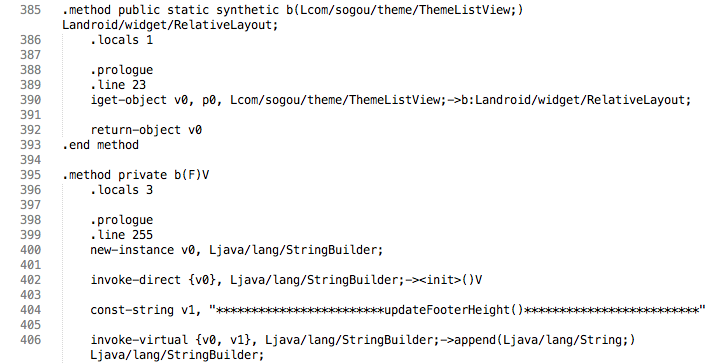
\includegraphics[width=5in]{figures/smali}
	\caption{搜狗输入法中\texttt{ThemeListView.smali}文件的部分代码。}
\end{figure}
因此需要将\texttt{.apk}程序包反编译,转化成可读的程序代码,该过程通常被称为逆向工程(Reverse Enigneering)\cite{chikofsky1990reverse}。通过逆向工程,可以对移动应用的源代码进行静态程序分析,获取内部功能信息。本文使用\textit{Apktool}\cite{apktool}工具对移动应用进行反编译操作,可以恢复移动应用中的程序层次结构。以搜狗输入法移动应用为例,反编译后的程序层次结构如图4-7所示,上方最左侧是搜狗输入法的根目录——程序包名\texttt{com.sohu.inputmethod.sogou},左侧第二列是第一级目录中的文件内容,其中\texttt{AndroidManifest.xml}是4.4.2节permissions特征存放的位置,\texttt{assets}文件夹包含了assets资源文件,\texttt{res}文件夹包含了resources资源文件。所有反编译后的程序源代码都存放在\texttt{smali}文件夹下,且以\texttt{.smali}的文件格式存储。图4-8展示了搜狗输入法\texttt{ThemeListView.smali}文件中的部分源代码,可以观察到,函数修饰符(\texttt{public/private})、函数参数(\texttt{Ljava/lang/String})、函数调用(\texttt{Landroid/widget/RelativeLayout},在4.4.2节中将讨论该类视图相关的函数)等都得到了恢复。利用反编译后的程序源代码,可以对移动应用进行视图和代码层面的分析,从而提取相关的功能特征,下节将详细讨论特征提取的方法。


\subsection{特征抽取}
本文基于视图的相似性计算方法,其动机来源于使用移动应用过程中的观察和发现。通常,人们仅仅通过查看移动应用的截图界面就能够快速辨别出两个移动应用是否相似。Viennot等\cite{viennot2014measurement}也曾提及过类似的观点。因此,本文将从移动应用视图的角度,分析其特征信息,下文将详细阐述视图特征提取过程。

\begin{figure}
	\centering
	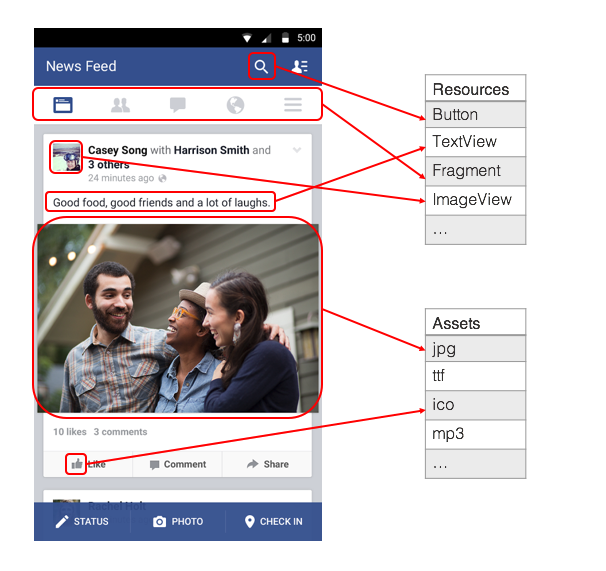
\includegraphics[width=5in]{figures/screenshot}
	\caption{Facebook移动应用中的resources和assets。左侧图片上的红色框表示Facebook移动应用所使用的resources和assets,右侧是其对应的具体列表。}
\end{figure}

在Android移动应用中,有两种主要的数据资源,分别为resources和assets。这两个数据资源存储了移动应用的视图信息,例如用户界面布局、图片、头像等。以Facebook移动应用为例,如图4-9所示,左侧部分是Facebook移动应用的用户界面,右侧则表示该移动应用中所使用的两种资源的列表。用户界面上标记的红色方框,且与右侧列表相连的列表,是Facebook移动应用中所使用的一些resources和assets资源。

Android平台上的resources资源以层次结构存储在称为\textbf{R}\cite{r}的Java类中。\textbf{R}文件是移动应用中存储界面布局resources资源名字(例如,\textit{Button}、\textit{EditText}、\textit{ListView}等)的一个基本文件。图4-10展示了一个\textbf{R}文件的例子,可以看到文件内存储了界面布局的resources名字以及对应的ID。这些resources名字对应了移动应用中相应的视图元素,如图4-10右侧红框中的\texttt{edit\_style1}是一个\textit{EditText}文本编辑框,\texttt{0x7f02000e}是其对应的ID。因此,本文通过\textbf{R}文件中的resources资源名,查找移动应用中使用对应资源的方法、函数等,从而识别相应的视图特征。本文使用4.4.1节中阐述的方法对移动应用进行逆向工程,然后对反编译后的程序代码进行分析,其代码形式如下:
\begin{center}
\texttt{Landroid/widget/ImageView;->setSelected(Z)}
\end{center}
\begin{figure}
	\centering
	\includegraphics[width=6.2in]{figures/R}
	\caption{移动应用中的\textbf{R}文件,其中包含了resources资源的名字和ID。右侧红框中给出了resources资源的一个例子,\texttt{edit\_style1}是一个resources资源的名字,\texttt{0x7f02000e}是该资源唯一编码的十六进制ID。}
\end{figure}
其中,代码的前半部分\texttt{android/widget/ImageView}表示对应代码所使用的类的名字,后半部分\texttt{setSelected(Z)}表示此函数的名字。此函数是由一个\textit{ImageView}的resources资源调用,因而可以据此将这一资源的使用情况作为resources特征,来表征移动应用的视图特征。因此,本文根据\textbf{R}文件中所列的所有resources资源名,对反编译后的源代码进行遍历,查找资源对应的调用函数,若调用了相应函数,则标记为1。从程序代码中识别的函数调用,将作为resources资源特征,用$\textbf{r}_i = \{r_{i,1}, r_{i,2}, ...\}$表示移动应用所使用的所有resources资源,其中$r_{i,1} \in \{0, 1\}$表示所调用的某一个resources相关的函数。

\begin{figure}
	\centering
	\includegraphics[width=3.2in]{figures/assets}
	\caption{移动应用中的assets文件夹,文件夹中包含了移动应用所有的assets资源文件,如移动应用启动界面的图片\texttt{ic\_launcher.png}。}
\end{figure}

对于移动应用中所使用的assets资源,可以从图4-11中观察到,该类资源是存储在移动应用程序包下的assets文件夹中。assets资源文件包括图片、音频、视频等,其通常会根据具体资源的内容进行命名,例如图4-11中的移动应用启动界面图片\texttt{ic\_launcher.png}。不同移动应用在使用assets资源时,在命名方式和文件格式上具有一定的相似性。因此本文利用这一特点,对assets资源文件进行分析,使用情况相近的移动应用通常表现出一定的相似性。所有静态的assets资源(本文暂时不考虑动态加载的资源数据)都包含在移动应用的程序包中,因此通过对\texttt{.apk}文件反编译后,可以从程序包中完全恢复其所使用的assets文件列表。本文将这些资源文件作为assets资源特征,用$\textbf{e}_i = \{e_{i,1}, e_{i,2}, ...\}$来表示移动应用所使用的所有assets资源,其中$e_{i,1} \in \{0, 1\}$表示所使用的某一个assets资源文件。

以上两类资源resources和assets是本文主要考虑的与移动应用视图相关的特征信息,可以用来表征移动应用视图以及程度代码层面的信息。为了充分利用移动应用程序包内的数据,本文同时对移动应用的permissions权限进行特征抽取。Permissions\cite{permission}是Android系统用以维护系统和用户安全的权限管理架构。由于移动设备不同于传统的个人计算机,其包含更多的物理资源(如全球定位系统、三轴振动仪等)和用户信息(如通讯录、银行卡密码等),恶意的移动应用可以通过获取这些资源和信息,从中获得非法利益,影响用户的正常使用和日常生活。为此,Android系统提供了permissions权限管理架构,用以管控这些敏感资源和信息,任何需要访问和使用相应资源的移动应用,需要主动向用户申请,并在\textit{AndroidManifest}文件中进行声明。开发者可以申请使用的permissions一共有152个,在Android开发者页面\cite{permission}可以查看所有可用的permissions权限。不同的移动应用会根据自身的功能,申请相应的权限。因此,移动应用所使用的permissions权限,一定程度上表征了移动应用所使用的功能信息。图4-12是某一移动应用的\textit{AndroidManifest}文件,红框中是该移动应用所申请的permissions权限。permissions权限的格式通常如下所示:
\begin{center}
\texttt{android.permission.ACCESS\_NETWORK\_STATE}
\end{center}
\begin{figure}
	\centering
	\includegraphics[width=6in]{figures/permissions}
	\caption{\textit{AndroidManifest}文件中声明了permissions权限列表,permissions在声明时的格式一致,如图中红框所示。}
\end{figure}
其中,\texttt{ACCESS\_NETWORK\_STATE}为权限的名字,该权限表示移动应用可以读取移动设备的网络状态,例如是否连接网络,连接的是蜂窝网络还是无线网络(Wi-Fi)。本文将移动应用在\textit{AndroidManifest}文件声明的permissions抽取出来,作为权限特征集合,表示为$\textbf{p}_i = \{p_{i,1}, p_{i,2}, ..., p_{i,152}\}$,其中$p_{i,1} \in \{0, 1\}$表示移动应用声明了某一permission权限。


\subsection{相似性计算}
本文在4.4.2中一共提取了三种类型的特征:resources、assets和permissions,此三类特征分别用$\textbf{r}_i$、$\textbf{e}_i$和$\textbf{p}_i$向量表示。因此,移动应用视图向量可以表示为$\textbf{v}_i = \textbf{r}_i \cup \textbf{e}_i \cup \textbf{p}_i$。由4.4.2节可知,视图向量使用了布尔值作为每一维特征表示,因此计算视图向量间的相似性即比较两个集合的相关性。Jaccard系数(Jaccard index或Jaccard similarity coefficient)通常作为计算两个样本集合间相似性和差异性的统计方法。本文使用Jaccard系数来表示两个移动应用在视图上的相似性,具体计算公式如下:
\begin{equation}
f_{\mathit{Jac}}(\textbf{v}_i, \textbf{v}_j) 
= \frac{| \textbf{v}_i \cap \textbf{v}_j |}{| \textbf{v}_i \cup \textbf{v}_j |}
= \frac{| \textbf{v}_i \cap \textbf{v}_j |}{| \textbf{v}_i | + | \textbf{v}_j | - | \textbf{v}_i \cap \textbf{v}_j |}
\end{equation}
其中,$\textbf{v}_i$和$\textbf{v}_j$为移动应用的视图向量,$|\textbf{v}_i|$表示视图向量$\textbf{v}_i$的长度。$f_{\mathit{Jac}}(\textbf{v}_i, \textbf{v}_j)$的取值范围在$[0,1]$之间,$f_{\mathit{Jac}}$的值越大,则表示两个视图向量间的相似度越高,进而说明两个移动应用的功能更为相似。

本文根据移动应用视图信息提取的特征来计算视图向量间的相似性,计算所得的结果表征了不同的移动应用在视图层面的相似性,从而体现了移动应用间的相似程度。在第五章实验部分,本文将详细讨论视图相似性在第三方库推荐中的表现。



%%%%%%%%%%%%%%%%%%%%%%%%%%%%%%%%%%%%%%%
%-----------------------------------     移动应用聚类     --------------------------------------%
%%%%%%%%%%%%%%%%%%%%%%%%%%%%%%%%%%%%%%%
\section{移动应用聚类}
当对一个数据量很大的数据集进行操作时,通常需要通过聚类的方法来减少计算量。聚类算法可以将相似的数据项聚集到一起,如此可以使后续的计算在一个簇内完成,而簇的大小通常与整体的数据集相差2-3个数量级,这将大大降低计算复杂度、缩短计算时间长度。由于互联网上拥有上百万的移动应用,如果需要通过与所有移动应用比较来寻找相似移动应用,显得极为不切实际。为此,本文利用聚类算法的特性,提前将功能相似的移动应用聚集到同一簇中,以提交相似移动应用检测的效率。本文利用在4.3节和4.4节中提出的文本和视图相似性计算方法,对移动应用间的相似程度进行计算。因为在聚类过程中可能使用文本相似性、视图相似性,或是文本与视图结合的相似性,所以在本节中统一用$f(\mathbf{a}_i, \mathbf{a}_j)$来表示相似性计算方法,具体计算方法如下所示(参数$\mu$为文本与视图相似性间的比重):
\begin{equation}
f(\mathbf{a}_i, \mathbf{a}_j) =
\left\{\begin{matrix}
f(\mathbf{t}_i, \mathbf{t}_j) & \mathrm{textual \: features}, \\
f(\mathbf{v}_i, \mathbf{v}_j) & \mathrm{view \: features}, \\
\mu * f(\mathbf{t}_i, \mathbf{t}_j) + (1-\mu) * f(\mathbf{v}_i, \mathbf{v}_j) & \mathrm{textual \& view \: features}.
\end{matrix}\right.
\end{equation}

K-means算法\cite{hartigan1979algorithm}是最为常见的聚类算法之一,在计算机视觉\cite{ray1999determination}、自然语言处理\cite{lin2009phrase}、地质统计学\cite{honarkhah2010stochastic}等领域被广泛应用。K-means聚类算法的目标是将$n$个观察对象划分成$k$个簇,使得每个簇内的点与中心点的平均距离最小。在本文研究的对象中,移动应用间的相似性表征了互相间的距离,这与原始的k-means算法中点与点之间的距离类似。K-means算法的目标函数是最小化每个簇内点到中心点距离的总和,即在每个簇中,需要计算簇中心点到簇内其他点的距离,中心点可以是数据集中的点,也可以是计算所得且不在数据集中的中心位置。由于本文研究的对象是移动应用,在聚类过程中,中心点必须为实际存在的移动应用,因此需要对k-means算法的目标函数做一定的调整。本文以每个簇内所有移动应用与中心移动应用间的平均相似性作为簇的相似性,对移动应用进行聚类,平均相似性的计算公式如下所示:
\begin{equation}
\mathit{Sim} = \frac{1}{m} \sum_{\mathbf{a}_o, \mathbf{a}_i \in S} f(\mathbf{a}_o, \mathbf{a}_i)
\end{equation}
其中,$m$表示簇$S$中移动应用的数量,$\mathbf{a}_o$表示簇$S$中心移动应用的特征向量,$f(\cdot)$为\textbf{定义4.1}和公式(4-9)中的移动应用相似性计算方法,根据具体的特征类别(文本或视图)来计算相应的相似性。那么,k-means的目标函数可以调整为如下形式:
\begin{equation}
\underset{\mathcal{S}}{\arg \max} \sum_{l=1}^{k} \frac{1}{m} \sum_{\mathbf{a}_o, \mathbf{a}_i \in S_l} f(\mathbf{a}_o, \mathbf{a}_i)
\end{equation}
其中,$\mathcal{S}$表示$k$个簇的集合,$S_l$为第$l$个簇。由于移动应用间的相似值越大,表示相互间的相似程度越高,因此在目标函数中需要最大化$k$个簇的相似性总和。

在原k-means算法基础上,对其目标函数进行改造,可以适用于本文研究对象的聚类问题。然而,在目标函数中使用平均相似性,只考虑了簇的中心移动应用与簇内其他移动应用间的相似性,忽略了每一对移动应用间的两两相似情况,这可能会导致聚类偏差问题——每个簇有较小的均值,方差却很大。如果出现这样的情况,则并没有实现将相似的移动应用都聚到一个簇中。如图4-13所示,现有四个移动应用,其中$\mathsf{app_1}$、$\mathsf{app_2}$和$\mathsf{app_3}$是由平均相似性聚类而成的三个移动应用簇,其中$\mathsf{app_3}$为簇的中心。从图中观察可以发现,由于$\mathsf{app_4}$与中心移动应用的相似值(红色框)要小于$\mathsf{app_1}$与中心的相似值,导致在聚类过程中,$\mathsf{app_4}$被排除在外。
\begin{figure}
	\centering
	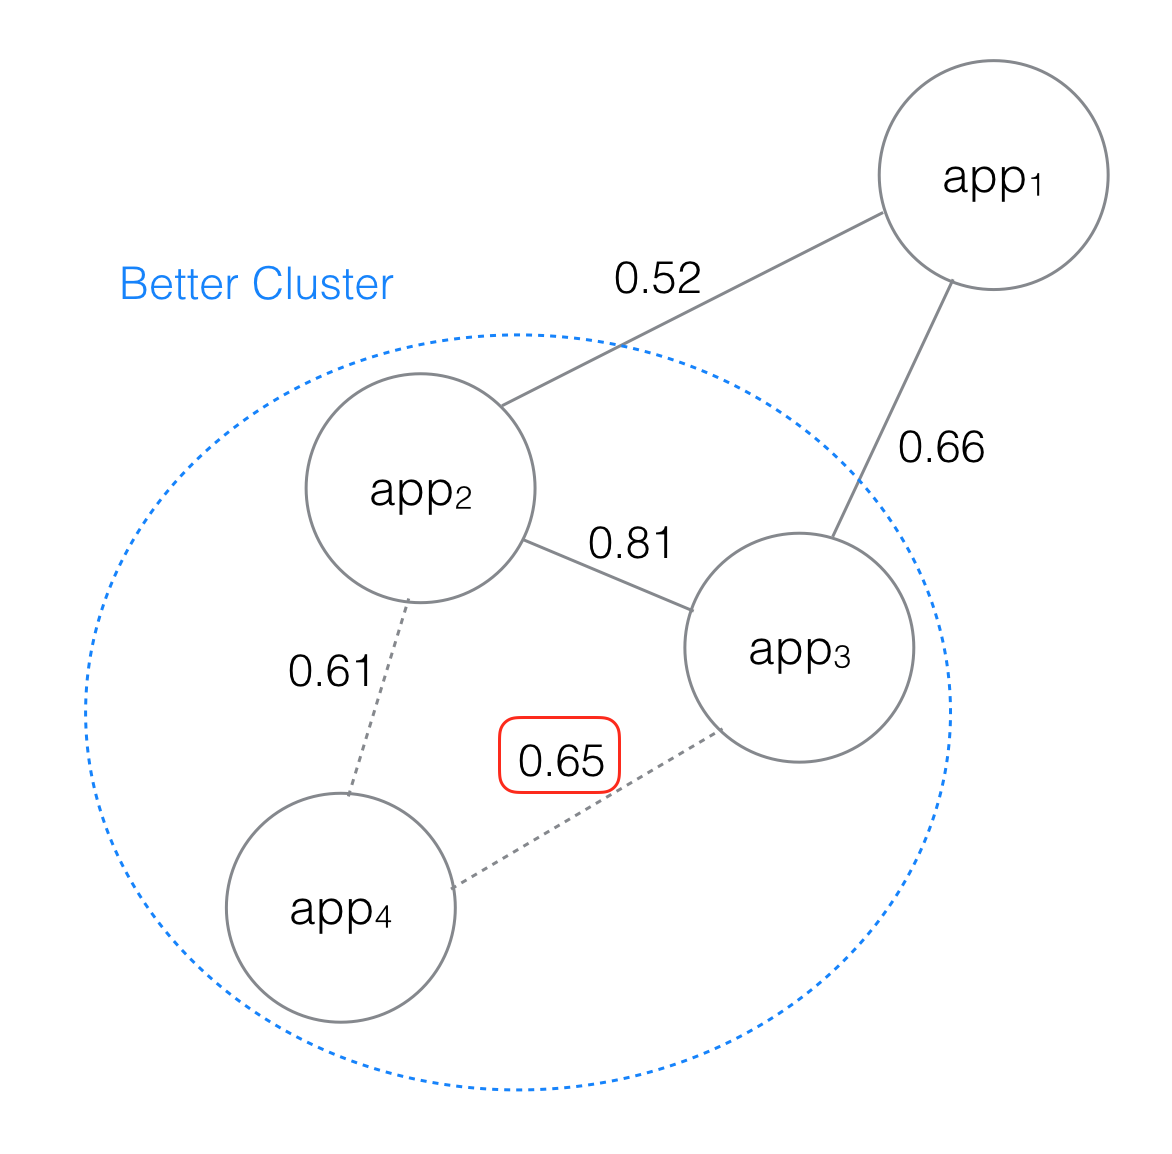
\includegraphics[width=4.8in]{figures/clustering}
	\caption{四个移动应用通过平均相似性聚类后的结果(实线连接)与可以更好的聚类结果(蓝色虚线圈)的比较。实线表示聚类后的连接关系,虚线表示可能的连接关系,连接线两侧的数据表示所连接的移动应用间的相似值。}
\end{figure}
通过观察可以发现的是,蓝色虚线圈所包括的三个移动应用,相互间更为相似。虽然$\mathsf{app_1}$被聚类在最终的簇中,但其于$\mathsf{app_2}$的相似性较其他移动应用要小得多,本不该被聚类在簇中。由于平均相似性忽略了$\mathsf{app_1}$和$\mathsf{app_2}$之间的相似性关系,导致最终的聚类结果差强人意。

凝聚式的层次聚类算法\cite{hierarchical}与k-means聚类算法不同,其将每个观察对象看作是单独的一个簇,通过不断合并距离最近的簇,最终达到聚类效果。该聚类算法考虑了观察对象之间的两两关系。其中,使用单连接法的凝聚式层次聚类,以最小距离作为聚类评判标准,将距离最小的簇合并。应用于移动应用聚类,则以最大相似性作为判别方法,具体公式如下:
\begin{equation}
\max \{ f(\mathbf{a}_x, \mathbf{a}_y) : \mathbf{a}_x \in \mathcal{X}, \mathbf{a}_y \in \mathcal{Y} \}
\end{equation}
其中,$\mathcal{X}$和$\mathcal{Y}$表示两个簇,$\mathbf{a}_x$和$\mathbf{a}_y$分别为簇$\mathcal{X}$和簇$\mathcal{Y}$内的移动应用,$f(\mathbf{a}_x, \mathbf{a}_y)$为移动应用间的相似性。从该聚类算法看,似乎可以解决k-means所遇到的问题——无法利用移动应用间的两两相似性,但实则仍具有局限性。以图4-13为例,四个移动应用初始均属于不同的簇($\{\mathsf{app_1}\}$,$\{\mathsf{app_2}\}$,$\{\mathsf{app_3}\}$,$\{\mathsf{app_4}\}$),需要计算两两相似性,将最相似的两个簇合并。使用单连接的方法进行操作,$\{\mathsf{app_2}\}$和$\{\mathsf{app_3}\}$间具有最大的相似性,因此将合并为同一个簇。此时,簇的情况为$\{\mathsf{app_1}\}$,$\{\mathsf{app_2}, \mathsf{app_3}\}$,$\{\mathsf{app_4}\}$。再次对各个簇进行两两相似性计算,使用公式(4-12)计算$\{\mathsf{app_1}\}$和$\{\mathsf{app_2}, \mathsf{app_3}\}$之间所得的值为0.66,而$\{\mathsf{app_4}\}$和$\{\mathsf{app_2}, \mathsf{app_3}\}$间的结果为0.65。显然,$\{\mathsf{app_1}\}$将会与$\{\mathsf{app_2}, \mathsf{app_3}\}$合并为一个簇,依旧无法获得最佳的聚类效果。

为了解决上述出现的问题和挑战,本文将簇内移动应用对的最小相似性作为簇的相似性表征,从而保证簇内真实的聚类情况。基于此,本文对现有的聚类算法进行优化和改进,提出了新的聚类算法,命名为k-min聚类算法。下面对k-min聚类算法进行定义:
\begin{definition}[K-min聚类算法]
给定一组移动应用$(\mathbf{a}_1, \mathbf{a}_2, ..., \mathbf{a}_n) \in \mathcal{A}$,其中每个移动应用为$\mathbf{a}_i = \{\mathbf{t}_i, \mathbf{v}_i\}$包含文本或视图的向量,k-min聚类算法的目标是将这$n$个移动应用分成$k(\leq n)$个簇$\mathcal{S} = \{S_1, S_2, ..., S_k\}$,且最大化移动应用对的相似性的最小值,即最优化以下目标函数:
\begin{equation}
\underset{\mathcal{S}}{\arg \max} \sum_{l=1}^{k} \mathcal{F}_l,
\end{equation}
\begin{equation}
\mathcal{F}_l = \min_{\mathbf{a}_i, \mathbf{a}_j \in S_l} f(\mathbf{a}_i, \mathbf{a}_j)
\end{equation}
其中,$\mathcal{F}_l$是簇$S_l$的相似值,$f(\mathbf{a}_i, \mathbf{a}_j)$为\textbf{定义4.1}中的相似性计算函数。
\end{definition}

本文提出的k-min聚类算法是用以对相似移动应用进行聚类的方法,该算法保证了每个簇都具有最大的簇内相似性和最小的簇间相似性。为了最优化\textbf{定义4.2}中的目标函数,本文引入了两个参数:参数$\varepsilon$用来控制聚类的精度,参数$\eta$用来控制迭代的次数。\textbf{算法4.1}中给出了k-min聚类算法的主要过程,包括以下四个步骤:

\begin{figure}[htb]
\centering
\begin{minipage}{.7\linewidth}
\begin{algorithm}[H]
	\small
	\caption{K-min聚类算法}
	\begin{algorithmic}[1]
	\Require
		\Statex $\mathcal{F}$ : Cluster Similarity
		\Statex $k$ : Cluster Number
		\Statex $\eta$ : Iteration Number
		\Statex $\varepsilon$ : Precision Control
	\Ensure
		\Statex $\mathcal{S}$ : Clusters
	\Statex
	\State $\mathcal{C} \leftarrow$ Random Apps
	\While {$\eta > 0$}
		\State $\Phi = True$
		\For {$i \leftarrow 1, k$}
			\State $\Delta = \mathcal{F}_i^{\eta} - \mathcal{F}_i^{(\eta+1)}$
			\If {$\Delta < 0$ or $\Delta > \varepsilon$}
				\State $\Phi = False$
				\State break
			\EndIf
		\EndFor
		\If {$\Phi$}
			\State break
		\Else
			\For {$i \leftarrow 1, k$}
				\State $\mathcal{C}_i = \underset{\mathbf{a}_x, \mathbf{a}_y \in S_i}{\arg \max \min} f(\mathbf{a}_x, \mathbf{a}_y)$
			\EndFor
		\EndIf
		\State $\eta = \eta - 1$\
	\EndWhile
	\end{algorithmic}
\end{algorithm}
\end{minipage}
\end{figure}

\begin{itemize}
\item
步骤1(1-3行):从移动应用集合$\mathcal{A}$中随机筛选出$k$个移动应用作为$k$个簇的初始中心移动应用。参数$\Phi$用以检查每次迭代后的结果,具体如下:
\begin{equation}
\Phi =
\left\{\begin{matrix}
True & \Delta > 0 \, \& \, \Delta < \varepsilon, \\
False & \mathrm{otherwise}.
\end{matrix}\right.
\end{equation}
其中,参数$\Delta$表示每次迭代后各簇相似性的变化情况,参数$\varepsilon$用以控制聚类算法的精度。本文将参数$\Phi$初始化为\textit{True};

\item
步骤2(4-10行):对每一簇,计算簇相似性的变化情况,如下:
\begin{equation}
\Delta = \mathcal{F}_l^{\eta} - \mathcal{F}_l^{(\eta+1)}
\end{equation}
其中,$\mathcal{F}_l^{(\eta+1)}$表示簇$S_l$在上一轮迭代中的簇相似性,$\mathcal{F}_l^{\eta}$则为当前轮迭代中的簇相似性。如果两轮迭代间簇相似性的差值小于参数$\varepsilon$的话,则聚类算法将结束;

\item
步骤3(11-17行):如果在新一轮的迭代中,簇相似性未发生大的变化,则算法将结束;不然,将对当前轮的各簇进行更新。具体而言,对当前轮迭代中的各簇,重新选择簇的中心移动应用,使得中心移动应用与簇内其他移动应用相似性的最小值最大化,具体公式如下:
\begin{equation}
\mathcal{C}_i = \underset{\mathbf{a}_x, \mathbf{a}_y \in S_i}{\arg \max \min} f(\mathbf{a}_x, \mathbf{a}_y)
\end{equation}
其中,$\mathcal{C}_i$为簇$S_i$的中心移动应用。对簇内任一移动应用$\mathbf{a}_x$而言,与其相似性最小的移动应用$\mathbf{a}_y$表征了移动应用$\mathbf{a}_x$所在范围(相似圈)的最边缘点,是本文最为关注的相似值。因此对这一相似值最大化,即使得移动应用$\mathbf{a}_x$相似圈最紧凑,以更小的相似半径(更大的相似值)包括簇内所有移动应用。

\item
步骤4(18-19行):对迭代参数$\eta$进行更新,从而进行下一轮的聚类迭代。
\end{itemize}

在k-min聚类算法中,参数$\varepsilon$和$\eta$用来控制聚类过程中整体的算法精度,保证能够在有限轮迭代中获得最优的聚类结果。通常而言,更大的$\varepsilon$参数和更小的$\eta$参数能够得到更好的聚类结果。根据移动应用的相似程度,对移动应用进行聚类操作,可以更快速更高效地找到与目标移动应用功能相近的其他已有移动应用,从而为后续的第三方库推荐做准备。对k-min聚类算法的表现将在第五章实验部分,与k-means和单连接的层次聚类算法进行对比实验,并详细讨论他们的优劣。



%%%%%%%%%%%%%%%%%%%%%%%%%%%%%%%%%%%%%%%
%-------------------------------------     第三方库推荐     ------------------------------------%
%%%%%%%%%%%%%%%%%%%%%%%%%%%%%%%%%%%%%%%
\section{第三方库推荐}
由于第三方库是由第三方开发者(个人或组织)开发并维护的,因此无法保证这些第三方库的质量优劣。如果移动应用开发者采用了质量较差的第三方库,不仅不能提高移动应用的用户体验,反而会减低其体验效果,甚至影响开发者声誉。为解决这一问题,则需要从移动应用开发者处收集对所使用的第三方库的反馈信息,以获取更多实际使用中可能存在的问题,为其他开发者提供参考和借鉴。本文通过分析评分较高的移动应用所使用的第三方库情况来解决这一问题。换而言之,评分较高的移动应用从其用户评分情况来看,可以认为其具有较好的质量。而分析这些质量较高的移动应用所使用的第三方库,能够相应得到质量较高的第三方库。此外,两个移动应用间的相似性显然非常重要,因为这表征了他们功能间的相似程度。

本文提出的TV-LibRec第三方库推荐算法充分利用了移动应用间的相似性,以及每个移动应用本身的质量(用户评分)。本文在4.3节和4.4节中分别讨论的移动应用文本和视图的特征,以及不同移动应用间相似性的计算方法。由以上两种相似性计算方法计算所得的移动应用具有很强的功能关联性,因此开发者采用这些相似移动应用中所使用的第三方库显得合情合理。此外,互联网上的移动应用有上百万之多,其质量良莠不齐,如果使用低质量的第三方库,则会对开发者产生不良影响。所以,需要考虑移动应用本身的质量情况,本文采用用户评分来衡量这一影响因素。因此,在为开发者推荐第三方库时,首先要根据开发者的需求寻找与之相关的相似移动应用,且同时考虑这些相似移动应用的评分情况。其次,将找到的相似移动应用中所使用的第三方库抽取出来,分析获得最为常用且质量最高的第三方库,为开发者推荐最合适的第三方库。本文在4.5节中对相似移动应用进行了聚类操作,可以基于此定位开发者的目标簇,从而使用top-z筛选方法选择与开发者期望最接近的若干个相似移动应用。本文对top-z筛选方法作如下定义:
\begin{definition}[Top-z筛选方法]
给定一组移动应用$(\mathbf{a}_1, \mathbf{a}_2, ..., \mathbf{a}_m) \in S$,top-z筛选方法的目的是从移动应用集合$S$中找到与开发者需求移动应用$\mathbf{a}_t$最相关的$z(\leq m)$个移动应用,其目标函数为:
\begin{equation}
\mathcal{L} = \{\mathbf{a}_i | i \leq z, \mathbf{a}_i \in \underset{S}{\arg sort} (D(\mathbf{a}_t, \mathbf{a}_j) | \mathbf{a}_j \in S, j \neq t)\}
\end{equation}
\begin{equation}
D(\mathbf{a}_t, \mathbf{a}_j) = \theta f(\mathbf{a}_t, \mathbf{a}_j) +  (1-\theta) d(\mathbf{a}_j)
\end{equation}
\begin{equation}
d(\mathbf{a}_j) = \frac{rating\_of\_app(\mathbf{a}_j)}{5.0}
\end{equation}
其中,函数$sort(\cdot)$将簇内的所有移动应用根据关系函数$D(\cdot)$的计算值按逆序排列。关系函数$D(\cdot)$表征了簇内移动应用与目标移动应用间的功能关系,由他们间的相似性函数$f(\cdot)$和移动应用质量$d(\cdot)$共同决定。关系函数$D(\cdot)$的值越大,则表示簇内移动应用$\mathbf{a}_j$与目标移动应用$\mathbf{a}_t$的功能关系越紧密。函数$d(\cdot)$表示移动应用的质量,用移动应用的实际评分除以最高评分五星,从而表示移动应用在用户评价中的质量表现。参数$\theta$用以权衡移动应用相似性与质量的比重。
\end{definition}

Top-z筛选方法根据与目标移动应用的关系度对簇内移动应用进行排序,从而给出了一个筛选后的移动应用候选列表。候选列表中的移动应用都具有较高的质量,且与目标移动应用相似性较高,因而从此列表移动应用中抽取的第三方库,可以推荐给开发者使用。移动应用间的相似性表征了他们之间的功能关系,亦包含了其使用的第三方库的功能信息。因为需要为开发者推荐合适的第三方库,即包含开发者所需功能的第三方库,所以需从其他移动应用所使用的第三方库中筛选出合适功能的第三方库。移动应用间的相似性一定程度上表征了这一关系,所以本文将该相似性引入第三方库筛选中。由于候选列表中的移动应用均具有较高的质量,因此在第三方库推荐过程中,本文将主要考虑移动应用相似性这一影响因子。就推荐给目标移动应用的每个候选第三方库,本文为之计算推荐分数:
\begin{equation}
\Omega = \frac{1}{z} \sum_{\substack{\mathbf{a}_i \in \mathcal{L} \\ \mathbf{a}_i \neq \mathbf{a}_t}} f(\mathbf{a}_t, \mathbf{a}_i) \cdot I
\end{equation}
其中,参数$z$为移动应用候选列表的大小,$f(\mathbf{a}_t, \mathbf{a}_i)$为目标移动应用$\mathbf{a}_t$与候选移动应用$\mathbf{a}_i$间的相似性,相似性计算方法如公式(4-9)所示。$I \in \{0,1\}$为指示参数,表示候选移动应用$\mathbf{a}_i$是否使用某一第三方库。如果$I = 0$,则表示候选移动应用未使用相应的第三方库,说明该第三方库可能不适合目标移动应用。基于此计算的推荐分数,表征了第三方库在候选移动应用中的使用率,从而说明相应第三方库的流行程度和质量。此外,本文还将移动应用的相似性加入到推荐分数计算过程,使得推荐分数$\Omega$同时具备了对第三方库功能和质量的评判,可以保证为开发者推荐的第三方库最合适且质量最高。本文引入参数$\alpha$来把控推荐过程,对于推荐分数大于$\alpha$的第三方库,将推荐给开发者。

至此,在4.5节聚类的基础上,本文充分利用了已有移动应用的功能和质量特征,从中筛选出符合开发者需求的第三方库,不仅保证了第三方库的功能性,亦考虑了第三方库的质量情况,解决了为开发者推荐优势合适的第三方库的研究问题。



%%%%%%%%%%%%%%%%%%%%%%%%%%%%%%%%%%%%%%%
%----------------------------------------     本章小结     ---------------------------------------%
%%%%%%%%%%%%%%%%%%%%%%%%%%%%%%%%%%%%%%%
\section{本章小结}
本章对本文所研究的问题——为移动应用开发者推荐优质合适的第三方库——作了具体定义,明确了本文研究问题的目标。针对本文的研究问题,本章从移动应用开发流程的两个阶段,提出了切实有效的解决方案。本文所提出的TV-LibRec算法框架一共分为了三个部分:首先,从移动应用中提取了能表征其功能的特征,并以此来计算移动应用间的相似性;然后,利用移动应用间的相似性,对功能相近的移动应用进行聚类操作;最后,在聚类后的簇中搜寻最符合开发者需求的第三方库,进而推荐给开发者使用。

本章针对移动应用相似性计算问题,分别从文本和视图两个数据层面,提出了可行的计算方法。移动应用描述信息是开发者对所开发的移动应用的功能描述文字,其包含了移动应用最基本的功能信息。因此,本文利用描述文本中的相关信息,从中提取表征移动应用功能的特征向量。本章详细介绍了本文对描述文本数据的处理过程,并阐述了doc2vec模型从文本到特征向量的转化过程。在文本特征向量的基础上,本章给出了针对文本特征的两种相似性计算方法:皮尔森相关系数和余弦相似度。本文亦从移动应用视图角度对功能特征进行抽取。本章详细阐述了针对移动应用的逆向工程方法,从而获得移动应用程序包的程序代码数据。在此基础上,本章介绍了移动应用中两种与视图相关的资源文件:resources和assets。此两类资源结合代码层数据,充分表征了移动应用的视图特征。本章同时利用了Android系统中的权限管理架构,即permissions特征,来对移动应用在敏感资源使用上的特征进行描述。综合三类移动应用内部的资源特征,本章给出了基于Jaccard系数的相似性计算方法,用以表征移动应用在视图层面的相似性。

在相似移动应用基础上,本章详细阐述了对其的聚类算法。本章首先考察了常用聚类算法k-means和单连接的层次聚类算法在本文问题上的适用性,并对其目标函数作相应调整,以适用于移动应用的聚类。本章详细分析了k-means和单连接的层次聚类算法在本文研究中的问题,并对该问题提出了相应的解决方法。为此,本章提出了一种针对移动应用聚类问题的新聚类算法k-min算法,该算法充分利用了任意两个移动应用间的相似性,从而解决了k-means和单连接的层次聚类算法在移动应用聚类过程遇到的问题和挑战。

最后,本章就本文研究问题,给出了可行的第三方库推荐算法。在相似移动应用聚类的基础上,本章针对开发者所需的目标移动应用,定位其所在的移动应用簇。推荐算法充分利用了移动应用相似性所表征的功能特征,以及移动应用评分所表征的应用质量,筛选了一个候选移动应用列表。该列表中的移动应用都具备高相似性、高质量的特点,分析并抽取其所使用的第三方库,可以确定适合开发者需求的第三方库。因此,本章将候选列表中的移动应用所使用的第三方库一一分析,并结合其相似性,计算第三方库的推荐分数。分数较高的第三方库则推荐给开发者使用。

本章对本文研究的问题作了深入分析和探讨,提出了基于文本和视图的TV-LibRec第三方库推荐算法。TV-LibRec充分利用了移动应用在文本和视图两个层次的相似性,并优化了已有的聚类算法,从而为开发者推荐优质合适的第三方库。